\documentclass[10pt]{article}
\usepackage[utf8]{inputenc}
\usepackage{url}
\usepackage{hyperref}
\usepackage{amsmath}
\usepackage{amsfonts}
\usepackage{amssymb}
\usepackage{graphicx}
\graphicspath{ {./images/} }
\usepackage{float}
\usepackage{lipsum}
\usepackage{sectsty}
\sectionfont{\centering}
\usepackage{multicol}
\usepackage{xcolor}
\usepackage{textcomp}
\usepackage{natbib}
\usepackage{graphicx}
\usepackage{listings}
\usepackage{xcolor}
\usepackage[font=small]{caption}
\addtolength{\abovecaptionskip}{-3mm}
\addtolength{\textfloatsep}{-5mm}
\setlength\columnsep{20pt}

\usepackage[a4paper,left=1.50cm, right=1.50cm, top=2cm, bottom=3cm]{geometry}


\author{}

\title{\Large{DAA Assignment - 2}}

\begin{document}
	
	\begin{center}
		{\Large \textbf{Design and Analysis of Algorithms}}\\
		\vspace{1em}
		{\Large \textbf{Assignment 2}}\\
		\vspace{1em}
		{\large Use divide and conquer to find stain in a cloth image.\\Take assumption for
cloth image by your own
}\\
		\vspace{1em}
		{\large Group 15}\\
		\vspace{1em}
		\large{Indian Institute of Information Technology, Allahabad}\\
		\vspace{1em}
		\large{Anirudh Gupta (IIT2019228), Navneet Bhole (IIT2019229), Eshan Vaid(IIT2019230)}\\
		\vspace{2.5em}
		
	\end{center}
	
\begin{multicols*}{2}

    \textbf{\emph{{Abstract}: This Paper introduces an algorithm to find stain in a cloth image using divide and conquer algorithm.}}\\
	
	\textbf{\emph{{Index Terms}: 2D Arrays, Divide and Conquer, Binary Search, Pixels, Image, Stain\\}}


\section*{I. INTRODUCTION}
 
A pixel is the smallest unit of a digital image or graphic that can be displayed and represented on a digital display device. A pixel is also known as a picture element (pix = picture, el = element).\\\\A pixel is represented by a dot or square on a computer monitor display screen. Pixels are the basic building blocks of a digital image or display and are created using geometric coordinates.\\\\Each of the pixels that represents an image stored inside a computer has a pixel value which describes how bright that pixel is, and/or what color it should be. \\\\For a grayscale images, the pixel value is a single number that represents the brightness of the pixel.\\\\The most common  pixel format is the byte image, where this number is stored as an 8-bit integer giving a range of possible values from 0 to 255.\\\\Typically zero is taken to be black, and 255 is taken to be white. Values in between make up the different shades of gray. The 256 possible gray intensity values are shown below.\\\\

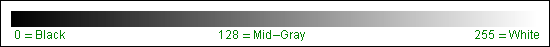
\includegraphics[width=7.7cm, height=1.1cm]{grayrange.png}\begin{center}\textbf{Figure 1:} The range of intensity values from 0 (black) to 255 (white).\end{center}
Consider the following 2D array of pixels\\\\Input:\\\\ arr[5][8] = [\\(250, 250, 250, 250, 250, 250, 250, 250)\\(250, 180, 150, 180, 250, 250, 250, 250)\\(250, 70, 0, 50, 250, 250, 250, 250)\\(250, 180, 140, 180, 250, 250, 250, 250)\\(250, 250, 250, 250, 250, 250, 250, 250)\\]\\\\Output: 0\\\\Above 2D Array is a matrix of pixels where each element is a pixel value. We have to find the stain. From Figure 1 we can infer that the element having the least pixel value will be the brightest so we have to find the least element i.e 0(Black) using Divide and Conquer algorithm.

\paragraph{Divide and Conquer}
Divide and Conquer is an algorithmic paradigm. The divide-and-conquer technique is the basis of efficient algorithms for many problems, such as sorting (e.g., quicksort, merge sort), multiplying large numbers (e.g., the Karatsuba algorithm),finding the closest pair of points. A typical Divide and Conquer algorithm solves a problem using following three steps. 
 The approach of divide and conquer generally follows three important aspects:
\begin{enumerate}
    \item\textbf{Divide:} Break the given problem into subproblems of same type.
    \item\textbf{Conquer:} Recursively solve these subproblems
    \item\textbf{Combine:} Appropriately combine the answers\\
\end{enumerate}Binary search is an example of Divide and Conquer algorithm. It has been used to solve above mentioned problem.\\\\The idea of binary search is to use the fact that each row of the above matrix is either constant or is first decreasing upto a point(which will be the least element of the row) then increasing (opposite of Bitonic sequence) and hence the time complexity is reduced to O(mlogn) where m = number of rows, n = number of columns.\\\\This report further contains -\\\\II. Algorithm Design\\III. Code\\IV. Illustration\\V. Algorithm Analysis\\VI. Conclusion\\VII. References\\VIII. Appendix


\section*{II. ALGORITHM DESIGN}
Consider the following 2D Array of pixels\\\\ arr[5][8] = [\\(250, 250, 250, 250, 250, 250, 250, 250)\\(250, 180, 150, 180, 250, 250, 250, 250)\\(250, 70, 0, 50, 250, 250, 250, 250)\\(250, 180, 140, 180, 250, 250, 250, 250)\\(250, 250, 250, 250, 250, 250, 250, 250)\\]\\\\A cloth image with above pixel distribution looks like below:\\

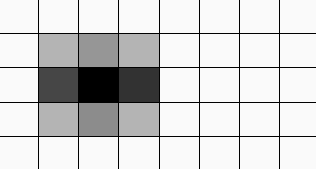
\includegraphics[width=8cm, height=5cm]{clothimage.png}\begin{center}\textbf{Figure 2:} Cloth image with above pixel distribution.\end{center}


\paragraph{Algorithmic Steps:}

Following are the cases that we consider in our algorithm\\\\Every time we go to the middle element and decide our next move based on the following cases\\\\Case 1:\\\\If the middle element is smaller than the element on the left side and also smaller than the element on the right side then it is the least element in that row.\\\\Case 2:\\\\If the middle element is not the least element, then check if the element on the left side is greater than the middle element then we will search on the right side of the middle element.\\\\Case 3:\\\\If the element on the right side is greater than the middle element then we will search on the left side of the middle element.\\\\Until the case 1 is satisfied and lo is lesser or equal to hi the above cycle is repeated.


\section*{III. CODE}
\lstset { %
    language=C++,
    backgroundcolor=\color{black!5},
    basicstyle=\footnotesize,
}

\begin{lstlisting}

FUNCTION findStain (arr, m, n) {

    pixel <- INT_MAX
    x
    y
    
    for i <- 0 to m - 1
    {
     
     lo <- 0
     hi <- n - 1
     
     while lo <= hi 
     {
       
       mid <- (lo + hi)/2
        
        if mid == 0 
        {   
            if arr[i][mid] < arr[i][mid+1]
            {
                if pixel > arr[i][mid] 
                {
	            pixel = arr[i][mid]
	            x = i
	            y = mid
	        } 
                break
            }
            else{
                lo = mid + 1
            }
        }
        
        else if mid == n - 1
        {
            if arr[i][mid] < arr[i][mid-1]
            {
                if pixel > arr[i][mid] 
                {
	            pixel = arr[i][mid]
	            x = i
	            y = mid
	        } 
                break
            }
            else
            {
                hi = mid - 1
            }
        }
        
        else if arr[i][mid] < arr[i][mid-1] && 
           arr[i][mid] < arr[i][mid+1] 
        {
          if pixel > arr[i][mid] 
          {
	            pixel = arr[i][mid]
	            x = i
	            y = mid
	   }
          break
        }
        
        else if arr[i][mid] < arr[i][mid-1]
         
          lo <- mid + 1
         
        else
        
          hi <- mid - 1
         
     }
     
    }  
    print x
    print y
    print pixel
}

FUNCTION main () {
    
    n, m 
    Input n
    Input m
    
    arr: 2D Array
    x
    
    for i <- 0 to m - 1
    {    
        for i <- k to n - 1
        {
           Input x
           arr[i][j] <- x
        }
    }    
    findStain (arr, m, n) 

}
\end{lstlisting}
Code Link: \url{https://ideone.com/Nxq928}
\section*{IV. ILLUSTRATION} 

Input:\\\\ arr[5][8] = [\\(250, 250, 250, 250, 250, 250, 250, 250)\\(250, 180, 150, 180, 250, 250, 250, 250)\\(250, 70, 0, 50, 250, 250, 250, 250)\\(250, 180, 140, 180, 250, 250, 250, 250)\\(250, 250, 250, 250, 250, 250, 250, 250)\\]\\\\Output: 0\\\\m(Number of rows) = 5\\\\n(Number of columns) = 8\\\\Initially pixel = INT\_MAX\\\\1. row = 0 lo = 0 hi = 7\\\\1a) while 0 $\leq$ 7\\

        mid = (0+7)/2 = 3\\

        arr[0][mid] = arr[0][3] = 250\\

        arr[0][mid-1] = arr[0][2] = 250\\

        arr[0][mid+1] = arr[0][4] = 250\\
        
        $\implies$ hi = mid - 1 = 3 - 1 = 2\\\\1b) while 0 $\leq$ 2\\
    
        mid = (0+2)/2 = 1\\

        arr[0][mid] = arr[0][1] = 250\\

        arr[0][mid-1] = arr[0][0] = 250\\

        arr[0][mid+1] = arr[0][2] = 250\\
        
       $\implies$ hi = mid - 1 = 1 - 1 = 0\\\\1c) while 0 $\leq$ 0\\
    
        mid = (0+0)/2 = 0\\

        arr[0][mid] = arr[0][0] = 250\\

        arr[0][mid+1] = arr[0][1] = 250\\
        
        $\implies$ hi = mid - 1 = 0 - 1 = -1\\
        
        STOP!\\
        
        pixel = INT\_MAX\\\\2. row = 1 lo = 0 hi = 7\\\\2a) while 0 $\leq$ 7\\

        mid = (0+7)/2 = 3\\

        arr[1][mid] = arr[1][3] = 180\\

        arr[1][mid-1] = arr[1][2] = 150\\

        arr[1][mid+1] = arr[1][4] = 250\\
        
        $\implies$ arr[1][mid] \textless arr[1][mid+1] (Case 3)\\
        
        $\implies$ hi = mid - 1 = 3 - 1 = 2\\\\2b) while 0 $\leq$ 2\\
    
        mid = (0+2)/2 = 1\\

        arr[1][mid] = arr[1][1] = 180\\

        arr[1][mid-1] = arr[1][0] = 250\\

        arr[1][mid+1] = arr[1][2] = 150\\
        
        $\implies$ arr[1][mid] \textless arr[1][mid-1] (Case 2)\\
        
        $\implies$ lo = mid + 1 = 1 + 1 = 2\\\\2c) while 2 $\leq$ 2\\
    
        mid = (2+2)/2 = 2\\

        arr[1][mid] = arr[1][2] = 150\\

        arr[1][mid+1] = arr[1][3] = 180\\
        
        arr[1][mid-1] = arr[1][1] = 180\\
        
        $\implies$arr[1][mid] \textless  arr[1][mid-1] \&\& arr[1][mid] \textless arr[1][mid+1] (Case 1)\\
    
        pixel = min(150,INT\_MAX) = 150\\
        
        STOP!\\\\3. row = 2 lo = 0 hi = 7\\\\3a) while 0 $\leq$ 7\\

        mid = (0+7)/2 = 3\\

        arr[2][mid] = arr[2][3] = 50\\

        arr[2][mid-1] = arr[2][2] = 0\\

        arr[2][mid+1] = arr[2][4] = 250\\
        
        $\implies$ arr[2][mid] \textless arr[2][mid+1] (Case 3)\\
        
        $\implies$ hi = mid - 1 = 3 - 1 = 2\\\\3b) while 0 $\leq$ 2\\
    
        mid = (0+2)/2 = 1\\

        arr[2][mid] = arr[2][1] = 70\\

        arr[2][mid-1] = arr[2][0] = 250\\

        arr[2][mid+1] = arr[2][2] = 0\\
        
        $\implies$ arr[2][mid] \textless arr[2][mid-1] (Case 2)\\
        
        $\implies$ lo = mid + 1 = 1 + 1 = 2\\\\3c) while 2 $\leq$ 2\\
    
        mid = (2+2)/2 = 2\\

        arr[2][mid] = arr[2][2] = 0\\

        arr[2][mid+1] = arr[2][3] = 50\\
        
        arr[2][mid-1] = arr[2][1] = 70\\
        
        $\implies$ arr[2][mid] \textless arr[2][mid-1] \&\& arr[2][mid] \textless arr[2][mid+1] (Case 1)\\
    
        pixel = min(0,150) = 0\\ 
        
        STOP!\\\\4. row = 3
   lo = 0
   hi = 7 \\\\4a) while 0 $\leq$ 7\\

        mid = (0+7)/2 = 3\\

        arr[3][mid] = arr[3][3] = 180\\

        arr[3][mid-1] = arr[3][2] = 140\\

        arr[3][mid+1] = arr[3][4] = 250\\
        
        $\implies$ arr[3][mid] \textless arr[3][mid+1] (Case 3)\\
        
        $\implies$ hi = mid - 1 = 3 - 1 = 2\\\\4b) while 0 $\leq$ 2\\
    
        mid = (0+2)/2 = 1\\

        arr[3][mid] = arr[3][1] = 180\\

        arr[3][mid-1] = arr[3][0] = 250\\

        arr[3][mid+1] = arr[3][2] = 140\\
        
        $\implies$ arr[3][mid] \textless arr[3][mid-1] (Case 2)\\
        
        $\implies$ lo = mid + 1 = 1 + 1 = 2\\\\4c) while 2 $\leq$ 2\\
    
        mid = (2+2)/2 = 2\\

        arr[3][mid] = arr[3][2] = 140\\

        arr[3][mid+1] = arr[3][3] = 180\\
        
        arr[3][mid-1] = arr[3][1] = 180\\
        
        $\implies$ arr[3][mid] \textless arr[3][mid-1] \&\& arr[3][mid] \textless arr[3][mid+1] (Case 1)\\
    
        pixel = min(140,0) = 0\\ 
        
        STOP!\\\\5. row = 0
   lo = 0
   hi = 7\\\\5a) while 0 $\leq$ 7\\

        mid = (0+7)/2 = 3\\

        arr[0][mid] = arr[0][3] = 250\\

        arr[0][mid-1] = arr[0][2] = 250\\

        arr[0][mid+1] = arr[0][4] = 250\\
        
        $\implies$ hi = mid - 1 = 3 - 1 = 2\\\\5b) while 0 $\leq$ 2\\
    
        mid = (0+2)/2 = 1\\

        arr[0][mid] = arr[0][1] = 250\\

        arr[0][mid-1] = arr[0][0] = 250\\

        arr[0][mid+1] = arr[0][2] = 250\\
        
        $\implies$ hi = mid - 1 = 1 - 1 = 0\\\\5c) while 0 $\leq$ 0\\
    
        mid = (0+0)/2 = 0\\

        arr[0][mid] = arr[0][0] = 250\\

        arr[0][mid+1] = arr[0][1] = 250\\
        
        $\implies$ hi = mid - 1 = 0 - 1 = -1\\
        
        STOP!\\\\6. return pixel = return 0
\section*{V.ALGORITHM ANALYSIS}

Time Complexity - Time complexity is the number of operations an algorithm performs to complete its task (considering that each operation takes the same amount of time). The algorithm that performs the task in the smallest number of operations is considered the most efficient one in terms of the time complexity.\\\\Space Complexity - The space complexity of an algorithm is the amount of memory space required to solve an instance of the computational problem as a function of characteristics of the input. It is the memory required by an algorithm until it executes completely.\\\\Time Complexity – We are iterating each row and then using binary search we are finding out the minimum element in the row so the overall time complexity would be O(mlogn) where m = number of rows, n = number of columns.\\\\Space Complexity – Since we have not used any extra data structure in our algorithm so the space complexity would be O(1).\\\\
Following is the time complexity graph in the case when number of rows is equal to the number of columns i.e m = n\\\\Time Complexity = mlogn = nlogn (m = n)\\\\
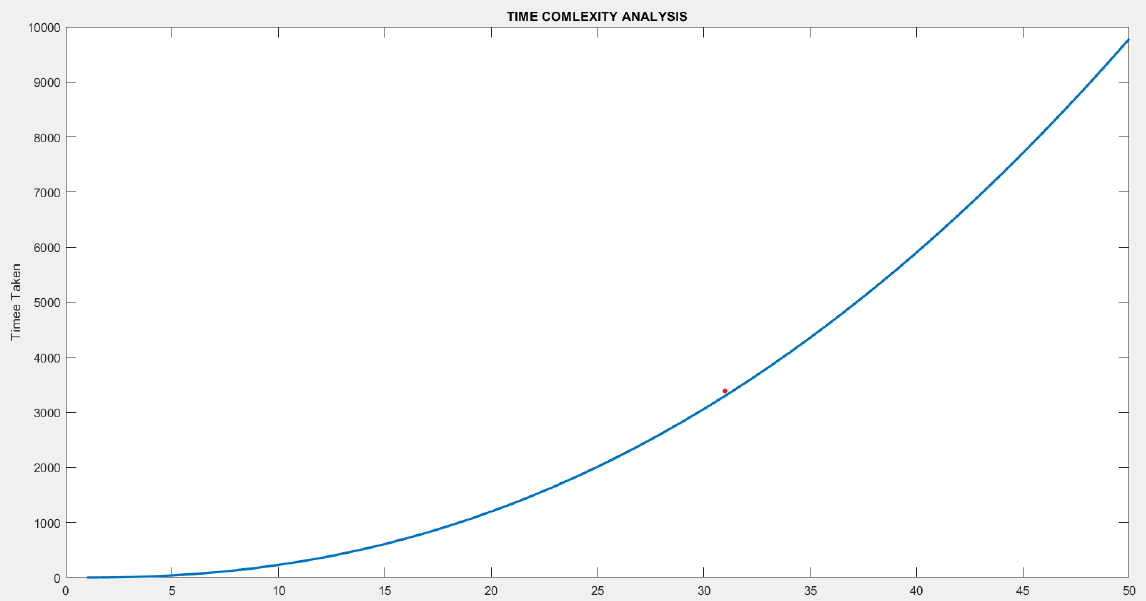
\includegraphics[width=\columnwidth, height=8cm]{Time Complexity.png}\begin{center}\textbf{Figure 3:} Time Complexity Graph\end{center}
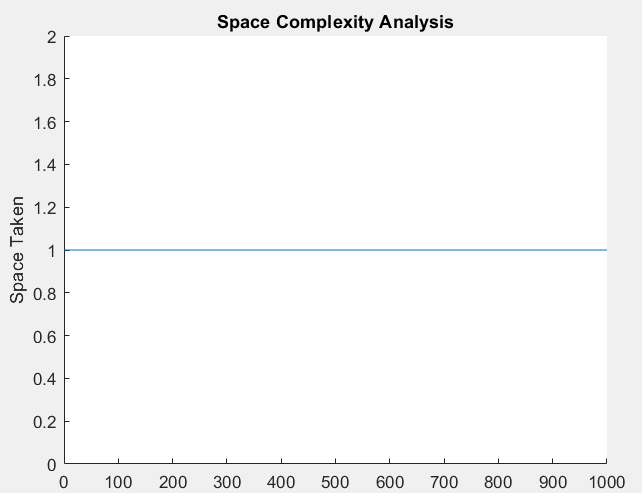
\includegraphics[width=\columnwidth, height=8cm]{Space Complexity.png}\begin{center}\textbf{Figure 4:} Space Complexity Graph\end{center}

\section*{VI.CONCLUSION}

This problem could be solved efficiently in O(mlogn) time complexity and O(1) space complexity using binary search algorithm where m = number of rows, n = number of columns.

\section*{VII. REFERENCES}

\begin{enumerate}
\item Introduction to Divide and Conquer Technique:\\
https://www.geeksforgeeks.org/divide-and-conquer-algorithm-introduction/
\item Find an element in Bitonic array\\
https://www.geeksforgeeks.org/find-element-bitonic-array/
\item Pixel Values\\
https://homepages.inf.ed.ac.uk/rbf/HIPR2/\\value.htm/
\item Digital Image Basics\\
https://www.whydomath.org/node/wavlets/\\imagebasics.html
\item Time Complexity\\
https://www.freecodecamp.org/news/time-\\complexity-of-algorithms/
\item Space Complexity\\
https://en.wikipedia.org/wiki/Space\_complexity
\end{enumerate}
\end{multicols*}

	
\end{document}